% VerdeAI gap-analysis pipeline — current (slot-filling) architecture.
% Same diagram/layout as the original state_compare-era figure; only the
% parts that actually changed are redrawn:
%   - "Compare State" -> "Slot Fill" (schema-driven extraction, still LLM)
%   - new "Score & Reconcile" node (score_clause — deterministic, no LLM)
%   - new "Aggregate Parents" node (worst-child-wins post-pass — deterministic)
% Everything else (ingestion row, retrieve/rerank, gap analyse, branches,
% legend) is unchanged from the original.
%
% Standalone: compiles on its own (e.g. on Overleaf) to a single cropped PDF/PNG.
\documentclass[tikz, border=6mm]{standalone}
\usetikzlibrary{shapes.geometric, arrows.meta, positioning, calc}

\definecolor{inkcolor}{HTML}{17241B}
\definecolor{mutedtext}{HTML}{4D5D4F}
\definecolor{terminalfill}{HTML}{F2F3EF}
\definecolor{iofill}{HTML}{B7C6DA}
\definecolor{decisionfill}{HTML}{E6D3A3}
\definecolor{processfill}{HTML}{BFD3BC}
\definecolor{aifill}{HTML}{CBB9D6}
\definecolor{reportfill}{HTML}{3E5C43}
\definecolor{newfill}{HTML}{9FC2B2}  % accent for the two genuinely-new nodes

\begin{document}
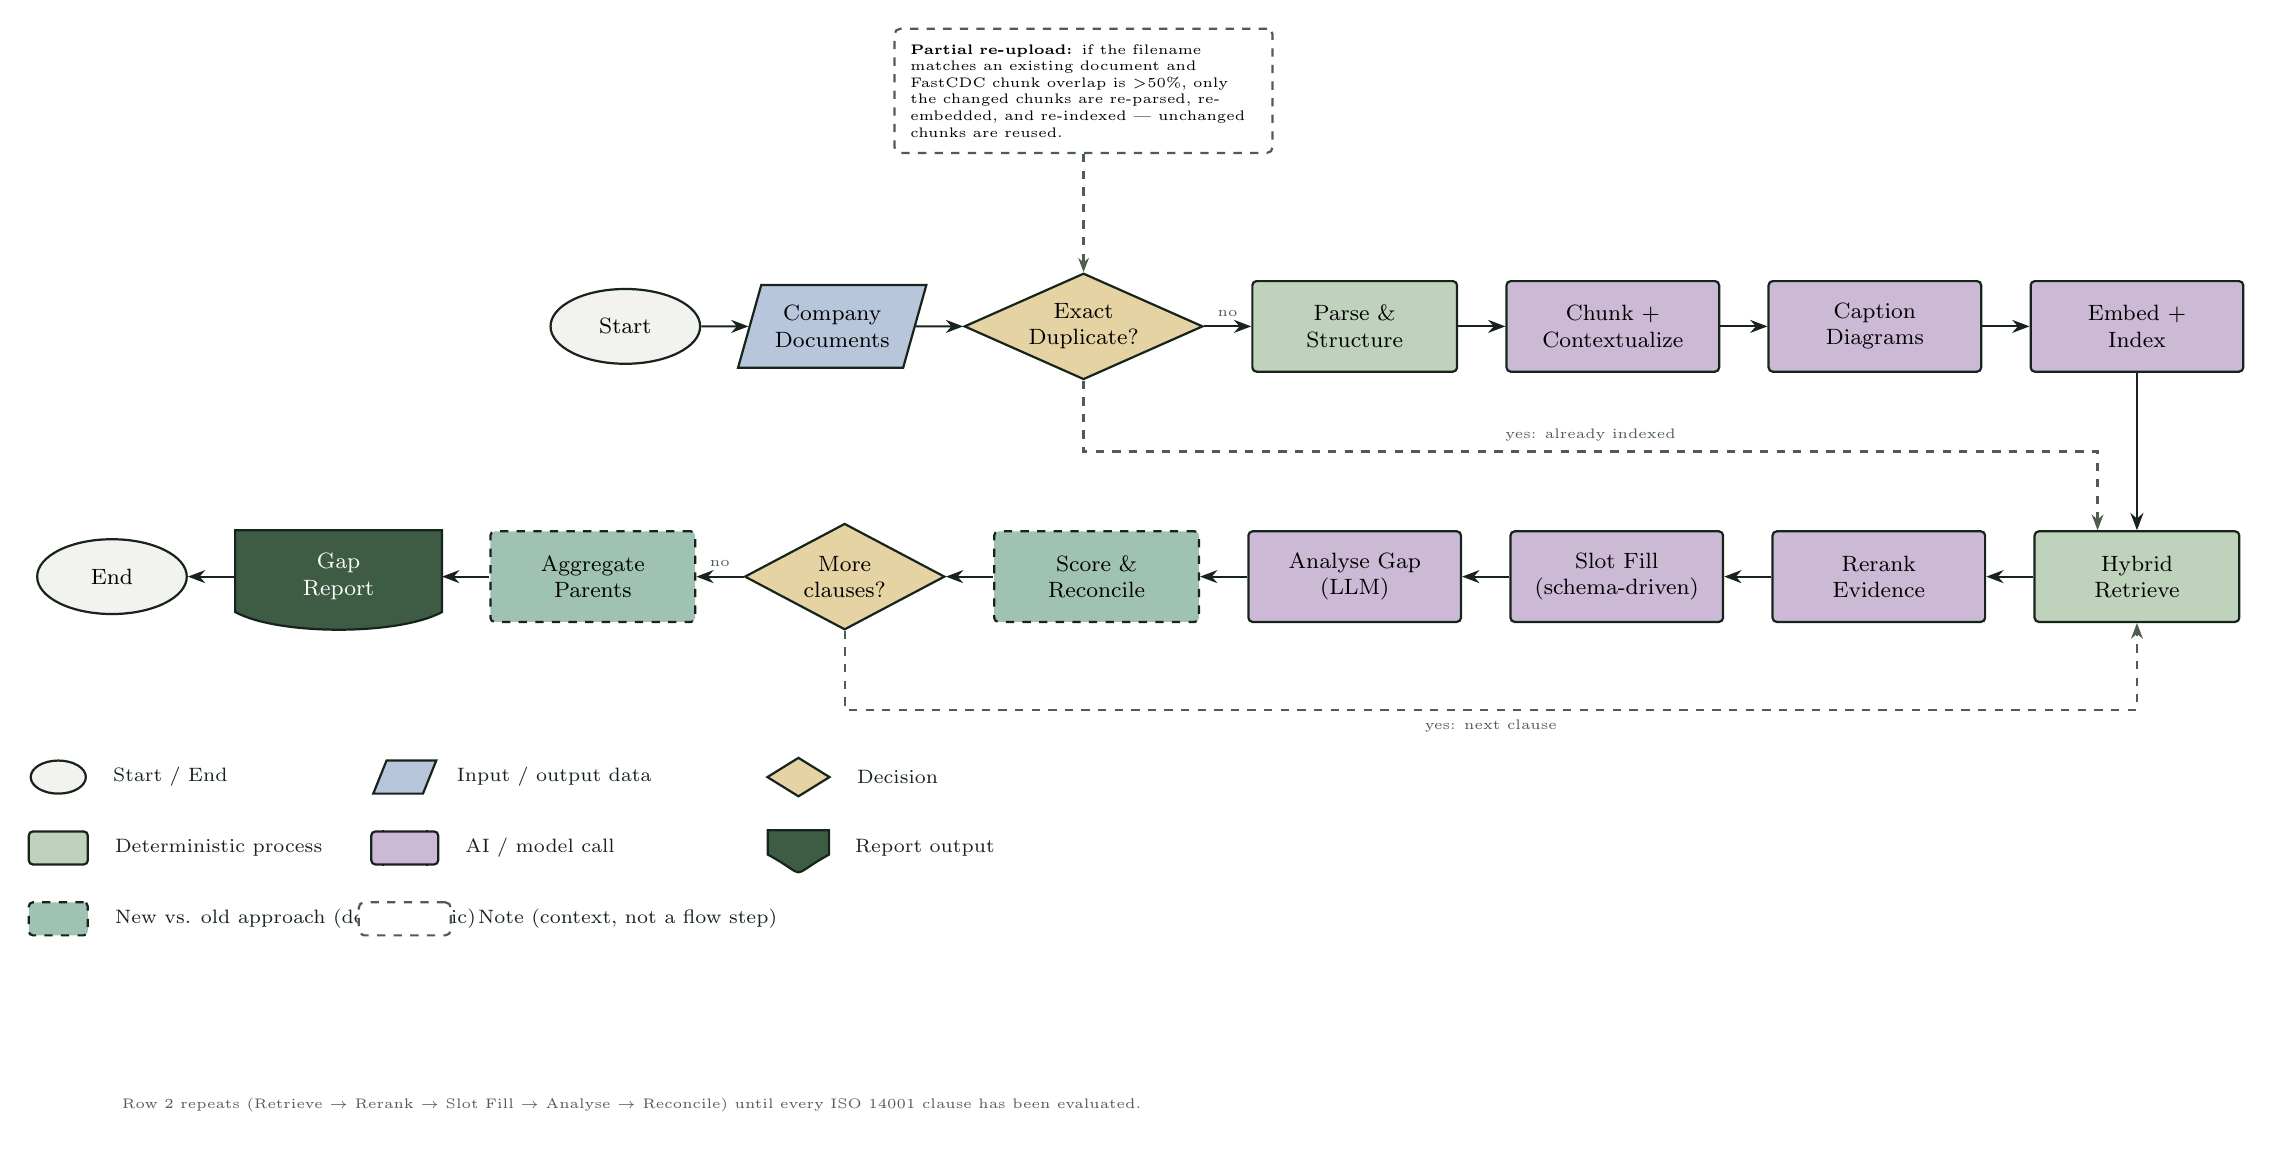
\begin{tikzpicture}[
  >=Stealth,
  every node/.style={font=\footnotesize},
  node distance=6mm and 6mm,
  align=center,
  thick,
]

\tikzset{
  terminal/.style={
    ellipse, draw=inkcolor, fill=terminalfill,
    minimum width=1.9cm, minimum height=0.95cm,
  },
  io/.style={
    trapezium, trapezium left angle=70, trapezium right angle=110,
    trapezium stretches=true,
    draw=inkcolor, fill=iofill,
    minimum width=2.4cm, minimum height=1.05cm,
  },
  decision/.style={
    diamond, draw=inkcolor, fill=decisionfill, aspect=2.4,
    inner sep=1pt, minimum width=2.5cm, minimum height=1.35cm,
  },
  process/.style={
    rectangle, rounded corners=1.5pt, draw=inkcolor, fill=processfill,
    minimum width=2.6cm, minimum height=1.15cm,
  },
  newprocess/.style={
    rectangle, rounded corners=1.5pt, draw=inkcolor, fill=newfill, dashed,
    minimum width=2.6cm, minimum height=1.15cm,
  },
  subprocess/.style={
    rectangle, rounded corners=1.5pt, draw=inkcolor, fill=aifill,
    minimum width=2.7cm, minimum height=1.15cm,
    append after command={
      \pgfextra{
        \draw[inkcolor]
          ($(\tikzlastnode.north west)!0.16cm!(\tikzlastnode.north east)$)
          -- ($(\tikzlastnode.south west)!0.16cm!(\tikzlastnode.south east)$);
        \draw[inkcolor]
          ($(\tikzlastnode.north east)!0.16cm!(\tikzlastnode.north west)$)
          -- ($(\tikzlastnode.south east)!0.16cm!(\tikzlastnode.south west)$);
      }
    },
  },
  flowline/.style={-{Stealth[length=2.2mm]}, inkcolor},
  branchline/.style={-{Stealth[length=2mm]}, mutedtext, dashed},
  annotation/.style={
    rectangle, rounded corners=2pt, draw=mutedtext, dashed, fill=white,
    text width=4.4cm, font=\tiny, align=left, inner sep=2mm,
  },
}

\newcommand{\documentshape}[2]{
  \draw[inkcolor, fill=reportfill]
    (#1.north west) -- (#1.north east)
    -- ($(#1.south east)+(0,0.14)$)
    .. controls ($(#1.south east)+(-0.55,-0.16)$) and ($(#1.south west)+(0.55,-0.16)$) ..
    ($(#1.south west)+(0,0.14)$) -- cycle;
  \node[text=white, align=center] at (#1) {#2};
}

% =================================================================
% ROW 1 — document ingestion & indexing (left to right) — UNCHANGED
% =================================================================
\node[terminal]                              (start)    {Start};
\node[io,         right=of start]            (docs)     {Company\\Documents};
\node[decision,   right=of docs]             (dup)      {Exact\\Duplicate?};
\node[process,    right=of dup]              (parse)    {Parse \&\\Structure};
\node[subprocess, right=of parse]            (chunk)    {Chunk +\\Contextualize};
\node[subprocess, right=of chunk]            (caption)  {Caption\\Diagrams};
\node[subprocess, right=of caption]          (embed)    {Embed +\\Index};

\node[annotation, above=15mm of dup] (note1)
  {\textbf{Partial re-upload:} if the filename matches an existing
  document and FastCDC chunk overlap is $>$50\%, only the changed
  chunks are re-parsed, re-embedded, and re-indexed --- unchanged
  chunks are reused.};
\draw[mutedtext, dashed, -{Stealth[length=1.8mm]}] (note1.south) -- (dup.north);

% =================================================================
% ROW 2 — per-clause gap analysis (right to left, below row 1)
% Only "compare" (renamed) and the two dashed nodes are new/changed.
% =================================================================
\node[process,    below=20mm of embed]       (retrieve) {Hybrid\\Retrieve};
\node[subprocess, left=of retrieve]          (rerank)   {Rerank\\Evidence};
\node[subprocess, left=of rerank]            (compare)  {Slot Fill\\(schema-driven)};
\node[subprocess, left=of compare]           (analyse)  {Analyse Gap\\(LLM)};
\node[newprocess, left=of analyse]           (reconcile){Score \&\\Reconcile};
\node[decision,   left=of reconcile]         (more)     {More\\clauses?};
\node[newprocess, left=of more]              (aggregate){Aggregate\\Parents};
\node[rectangle, minimum width=2.6cm, minimum height=1.15cm,
      left=of aggregate]                     (reportbox) {};
\node[terminal,   left=of reportbox]         (end)      {End};

% =================================================================
% Main flow — row 1
% =================================================================
\draw[flowline] (start) -- (docs);
\draw[flowline] (docs) -- (dup);
\draw[flowline] (dup) -- node[above, font=\tiny, text=mutedtext]{no} (parse);
\draw[flowline] (parse) -- (chunk);
\draw[flowline] (chunk) -- (caption);
\draw[flowline] (caption) -- (embed);

% bend: row 1 -> row 2
\draw[flowline] (embed.south) -- (retrieve.north);

% Main flow — row 2 (right to left)
\draw[flowline] (retrieve) -- (rerank);
\draw[flowline] (rerank) -- (compare);
\draw[flowline] (compare) -- (analyse);
\draw[flowline] (analyse) -- (reconcile);
\draw[flowline] (reconcile) -- (more);
\draw[flowline] (more) -- node[above, font=\tiny, text=mutedtext]{no} (aggregate);
\draw[flowline] (aggregate) -- (reportbox);
\draw[flowline] (reportbox) -- (end);

% =================================================================
% Branch 1 — duplicate short-circuit: skip straight to retrieval,
% the document's chunks are already indexed from a prior upload.
% =================================================================
\coordinate (bypassLane)  at ($(dup.south)+(0,-0.9)$);
\coordinate (bypassEntry) at ($(retrieve.north)+(-0.5,0)$);
\coordinate (bypassTurn)  at (bypassEntry |- bypassLane);
\draw[branchline]
  (dup.south) -- (bypassLane)
  -- node[above, font=\tiny, text=mutedtext]{yes: already indexed} (bypassTurn)
  -- (bypassEntry);

% =================================================================
% Branch 2 — loop back for the next ISO 14001 clause.
% =================================================================
\coordinate (loopLane)  at ($(more.south)+(0,-1.0)$);
\coordinate (loopEntry) at (retrieve.south);
\coordinate (loopTurn)  at (loopEntry |- loopLane);
\draw[branchline]
  (more.south) -- (loopLane)
  -- node[below, font=\tiny, text=mutedtext]{yes: next clause} (loopTurn)
  -- (loopEntry);

% document (report) shape, drawn on top of its placeholder node
\documentshape{reportbox}{Gap\\Report}

% =================================================================
% Legend
% =================================================================
\begin{scope}[shift={($(end.south west)+(0,-2.2)$)}]
  \node[terminal, minimum width=0.7cm, minimum height=0.42cm, font=\tiny] (l1) at (0,0) {};
  \node[right=2mm of l1, font=\scriptsize, text=inkcolor] {Start / End};

  \node[io, minimum width=0.8cm, minimum height=0.42cm, font=\tiny] (l2) at (4.4,0) {};
  \node[right=2mm of l2, font=\scriptsize, text=inkcolor] {Input / output data};

  \node[decision, minimum width=0.8cm, minimum height=0.5cm, font=\tiny] (l3) at (9.4,0) {};
  \node[right=2mm of l3, font=\scriptsize, text=inkcolor] {Decision};

  \node[process, minimum width=0.75cm, minimum height=0.42cm, font=\tiny] (l4) at (0,-0.9) {};
  \node[right=2mm of l4, font=\scriptsize, text=inkcolor] {Deterministic process};

  \node[subprocess, minimum width=0.85cm, minimum height=0.42cm, font=\tiny] (l5) at (4.4,-0.9) {};
  \node[right=2mm of l5, font=\scriptsize, text=inkcolor] {AI / model call};

  \node[rectangle, minimum width=0.75cm, minimum height=0.42cm] (l6) at (9.4,-0.9) {};
  \documentshape{l6}{}
  \node[right=2mm of l6, font=\scriptsize, text=inkcolor] {Report output};

  \node[newprocess, minimum width=0.75cm, minimum height=0.42cm, font=\tiny] (l7) at (0,-1.8) {};
  \node[right=2mm of l7, font=\scriptsize, text=inkcolor] {New vs. old approach (deterministic)};

  \node[annotation, text width=1.1cm, minimum height=0.42cm, inner sep=1pt,
        font=\tiny] (l8) at (4.4,-1.8) {};
  \node[right=2mm of l8, font=\scriptsize, text=inkcolor] {Note (context, not a flow step)};
\end{scope}

\node[font=\tiny, text=mutedtext, below=6mm of end, xshift=6.6cm, yshift=-5.4cm]
  {Row 2 repeats (Retrieve $\rightarrow$ Rerank $\rightarrow$ Slot Fill $\rightarrow$ Analyse
  $\rightarrow$ Reconcile) until every ISO 14001 clause has been evaluated.};

\end{tikzpicture}
\end{document}
